\chapter{Alternative SSA construction algorithms
   \Author{D. Das, U. Ramakrishna, and V. Sreedhar}}
\inputprogress
\graphicspath{{img/}{alternative_ssa_construction_algorithms/img/}{part1/alternative_ssa_construction_algorithms/img/}}


%\input defs


%\input defs


\section{Introduction}

The  placement  of $\phi$-functions
is an important step in the construction of Static Single Assignment 
(SSA) form~\cite{CytronEtAl91}.
 In SSA form
 every variable is assigned 
only once. At control flow merge points $\phi$-functions are added 
 to ensure that every use of a variable has exactly 
one definition. 
A $\phi$-function is of the form $x_n = \phi(x_0,x_1, x_2, \ldots, x_{n-1})$,
where $x_i$'s ($i = 0 \ldots n-1$) are a set of variables with static single assignment. 
Consider the example control flow graph where we have shown definitions and uses for 
a variable $x$. The SSA form for the variable $x$ is illustrated in Figure ~\ref{fig:cfg}(a). 
Notice $\phi$-functions
have been introduced at certain join (also called merge) nodes in the control flow graph.
In the rest of this chapter we will present three different approaches  for placing $\phi$-functions
at appropriate join nodes. Recall that SSA construction falls into two phases of $\phi$-placement and variable renaming. Here we present different approaches for the first phase for minimal SSA form. We first present Sreedhar and Gao's algorithm for
placing $\phi$-functions. Sreedhar and Gao's algorithm uses DJ graph representation of a CFG.
Then we will discuss the notion of merge set and merge relation, and present
Das and Ramakrishna's algorithm for placing $\phi$-functions based on merge relation and using DJ graph. Finally
we describe another approach for placing $\phi$-functions based on loop nesting forest proposed by Ramalingam.

\section{Basic Algorithm}
The original algorithm for placing $\phi$-functions
was based on first computing the dominance frontier  (DF) set for the given control flow graph.
The dominance frontier $DF(x)$ of a node $x$ is the set of all nodes 
 $z$ such that $x$ dominates a predecessor of $z$, without strictly dominating $z$.
For example, $DF(8)= \{ 6, 8 \}$ in Figure ~\ref{fig:cfg}(b). A straight forward algorithm for computing
DF for each node takes $O(N^2)$ (where $N$ is the number of nodes in the CFG) since the size of the full DF set in the worst case
can be $O(N^2)$.
Cytron et al.'s algorithm for the placement of $\phi$-functions consists of computing
iterated dominance frontier (IDF) for a set of all definition points (or nodes where
variables are defined). 
Let $N_{\alpha}$ be the set of nodes where variable $x$ are  defined.
Given that the dominance frontier for a set of nodes is just the
union of the DF of each node, we can compute $IDF(N_\alpha)$ as a limit of
the following recurrence equation (where $S$ is initially $N_\alpha$)
\begin{eqnarray*}
IDF_1(S) &=& DF(S) \\
IDF_{i+1} (S) &=& DF(S \cup IDF_i(S)) 
\end{eqnarray*}

A $\phi$-function is then placed at each join node in the  $IDF(N_{\alpha})$ set. 
Although Cytron et al.'s
algorithm works very well in practice, in the worst case the time complexity of $\phi$-placement algorithm for a single variable is quadratic in the number of nodes in the original control flow graph.




\section{Placing $\phi$-functions using DJ graphs}
Sreedhar and Gao 
proposed the first linear time algorithm for computing the IDF set without
the need for explicitly computing the full DF set. Sreedhar and Gao's original
algorithm was implemented using the DJ graph representation of CFG. A DJ graph
is a CFG augmented with dominator tree edges. An edge $x \edge{} y$, of the
CFG, which is not a dominator-tree edge, becomes a join(J) edge, referred as $x \edge{J} y$. The
DJ graph for the example CFG is also shown in Figure ~\ref{fig:cfg}(b). The CFG edge
$10 \edge{} 8$, which is not a dominator-tree edge becomes the J edge, $10 \edge{J} 8$.
Rather than explicitly
computing the DF set, Sreedhar and Gao's algorithm uses a DJ graph to compute the  $IDF(N_{\alpha})$ on-the-fly. Even though
 the time complexity of
Sreedhar and Gao's algorithm is linear in the size of the DJ graph, in practice it sometimes performs worse than the Cytron et al.
algorithm. The main reason for this is that in practice the size of the DF set is linear in the number of nodes in the CFG 
and sometimes smaller than the size of the DJ graph. 


\subsection{Key Observation} 
 
Now let us try to understand how to compute the DF for a single node using DJ graphs. 
Consider  the DJ graph shown in Figure~\ref{fig:cfg}(b). To compute $DF(8)$ we simply walk down the
dominator (D) tree edges from node 8 and identify all join (J) edges $x \edge{J} y$ such
the $y.level \leq 8.level$, where $level$ of a node is the depth of the node from the
root of the dominator tree. The $level$ of each node is also shown in Figure ~\ref{fig:cfg}(b).
For our example the J edges that satisfy this 
condition are $9 \edge{J} 6$ and $10 \edge{J} 8$. Therefore $DF(8) = \{6, 8\}$. To generalize the example, we can
compute the DF of a node $x$ using \\
\fbox{$DF(x) = \{y | z \in SubTree(x) \; \wedge \; z \edge{J} y \; \wedge \; y.level \leq x.level \}$}\\

    \begin{figure}[htb]
    \centerline{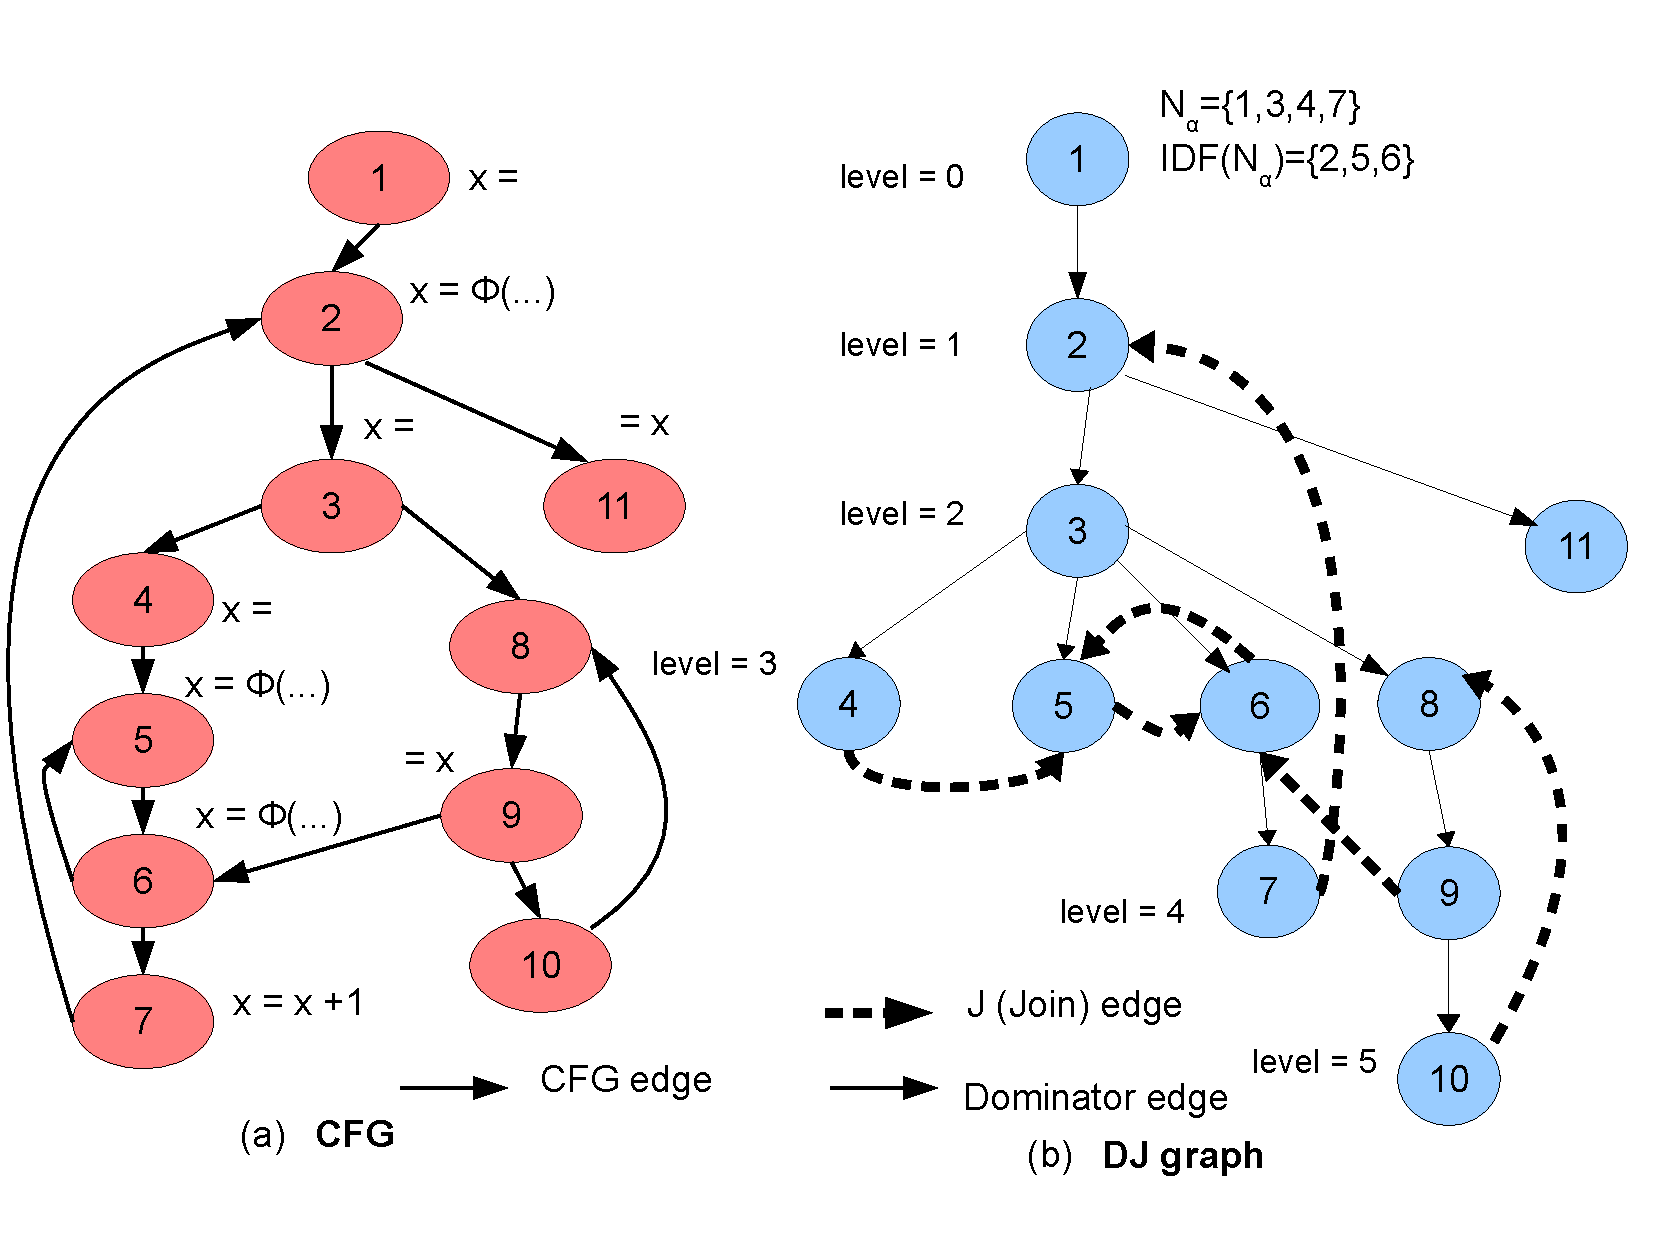
\includegraphics[scale=0.4]{cfglive_new.pdf}}
    \caption{A Motivating Example (a) CFG (b) DJ graph}
    \label{fig:cfg}
    \end{figure} 

Now we can extend the above idea to compute the IDF for a set of nodes, and hence the set of $\phi$-functions. This algorithm does not precompute DF. Given a set of initial nodes $N_{\alpha}$ to compute the relevant set of $\phi$-functions,
a key observation can be made. Let $y$ be an ancestor node of a node $x$ on the dominator tree. If $DF(x)$ has already been computed before the computation of $DF(y)$,  $DF(x)$ need not
be recomputed when computing $DF(y)$. This is because nodes reachable from $Subtree(x)$ are already in $DF(x)$. However, the reverse may not be true, and  therefore the order of the computation of DF is crucial.

To illustrate the key observation consider the example DJ graph in Figure \ref{fig:cfg}(b),
and let us compute $IDF(\{3,8\})$. Now supposing we start with node $3$ and compute 
$DF(3)$. The resulting DF set is $DF(3) = \{2\}$. 
Now supposing we next compute the DF set for node $8$, and the resulting set is
$DF(8) = \{6,8\}$. Notice here that we had already visited node $8$ and its subtree as part of visiting node $3$. We can avoid such duplicate visits by ordering the computation of DF set so that we first compute $DF(8)$ and then during the computation of $DF(3)$ we avoid visiting the sub-tree of
node $8$, and use the result $DF(8)$ that was previously computed. 

Thus, to compute $IDF(x,y)$ where $x$ is an ancestor of $y$ in the DJ graph one needs to compute: 

\begin{flalign*}
IDF(x,y) & = \{w|w \in DF(y) \wedge w.level \leq x.level\} \cup \\
          &  \{w|t \in Subtree(x) \setminus Subtree(y) \wedge t \edge{J} w \wedge w.level \leq x.level \}
%}. 
\end{flalign*}

Hence, from the equation, $IDF(3,8) = \{w|w \in DF(8) \wedge w.level \leq 3.level \} \cup \{w|t \in Subtree(3)\setminus Subtree(8) \wedge t \edge{J} w \wedge w.level \leq 3.level \}$, where the first part of the right hand side i.e. $\{w|w \in DF(8) \wedge w.level \leq 3.level \}$ is computed first to avoid duplicated effort. Since neither $6.level$ nor $8.level$ is lesser than $3.level$ none of the nodes in $DF(8)$ appear in $IDF(3,8)$. The nodes that appear in $Subtree(3)\setminus Subtree(8)$ are $4, 5, 6, 7$. From these only $7 \edge{J} 2$ has a target node $2$ such that $2.level \leq 3.level$. Hence $IDF(3,8)$ will include only node $2$ without duplicate visits to node $8$.

In the next section
we present the Sreedhar and Gao's algorithm based on the above key observation.


\subsection{Main Algorithm}

In this section we present Sreedhar and Gao's algorithm. Let $x.level$ be the
depth of the node from the root node with $root.level= 0$. To ensure that the nodes
are processed according to the first key observation we use  a simple 
 array of sets $OrderedBucket$, and two functions defined over the array of sets:
(1) InsertNode($n$) that inserts the node $n$ in the set $OrderedBucket[n.level]$, and
(2) GetNode() that returns a node from the $OrderedBucket$ with highest level number. 
The complete algorithm is shown in Figure~\ref{F:IDFMain}.

\begin{figure}[!ht]
\centering
\begin{minipage}[t]{5in}
\noindent{\bf Input:} A DJ graph representation of a program and $N_{\alpha}$.
\noindent{\bf Output:} The set $IDF(N_{\alpha})$.

Procedure IDFMain(Set $N_{\alpha}$) 
\{
\begin{code}
\x1 $IDF = \{ \}$;
\x1 {\bf foreach} ( node $x \in  N_{\alpha}$) {\bf do}
\x2    InsertNode($x$);
\x1 {\bf end for}
\x1 {\bf while} (($z = GetNode()) \neq NULL$)  \label{C:get}
\x2   $croot = z$;
 \x2  $z.visited = true$ ;
 \x2  Visit($z$);
\x1 {\bf end while}
\end{code}
\} 

Procedure Visit($x$)
\{
\begin{code}
\x1 {\bf foreach} (node $y \in  Succ(x)$) {\bf do}
\x2  {\bf if} ($x \edge{} y$ is a  J edge) {\bf then}
\x3   {\bf if} ($y.level \leq croot.level$) {\bf then}

\x4     {\bf if} ($y \not \in IDF$) {\bf then}
\x5        $IDF = IDF \cup {y}$;   \label{C:idf}
\x5        {\bf if} ($y \not  \in N_{\alpha}$) {\bf then}
\x6          InsertNode($y$); \label{C:insert}
\x5        {\bf endif}
\x4     {\bf end if}
\x3  {\bf end if}
\x2 {\bf else} // visit D edges 
\x3   {\bf if} ($y.visited == false $) {\bf then}
\x4    $y.visited = true$;
\x4    // if($y.boundary == false$)   \label{C:cached}
\x5     Visit($y$); \label{C:dedges}
%\x4     Visit($y$); \label{C:dedges}
\x4 // {\bf end if}
\x3   {\bf end if}
\x2  {\bf end if}
\x1 {\bf end for}
\end{code}
\} 
\end{minipage}
\caption{Sreedhar and Gao's algorithm for computing IDF set.}
\label{F:IDFMain}
\end{figure}

First we insert all nodes in $N_{\alpha}$ in the $OrderedBucket$. The nodes are processed
in a bottom-up fashion over the dominator tree from highest node level to least node level
(step ~\ref{C:get}). The procedure Visit($x$) essentially walks down the  DJ graph 
and identifies candidate J edges whose destination node are in the $IDF$ set (step \ref{C:idf}).
Notice that at step \ref{C:insert} a node is inserted in the {\it OrderedBucket} if it was
never inserted before. Finally at step \ref{C:dedges} we continue to process the nodes
in the sub-tree by visiting over the D edges. When the algorithm terminates the 
set $IDF$ will contain the IDF set for the initial $N_{\alpha}$.

    \begin{figure}[htb]
    \centerline{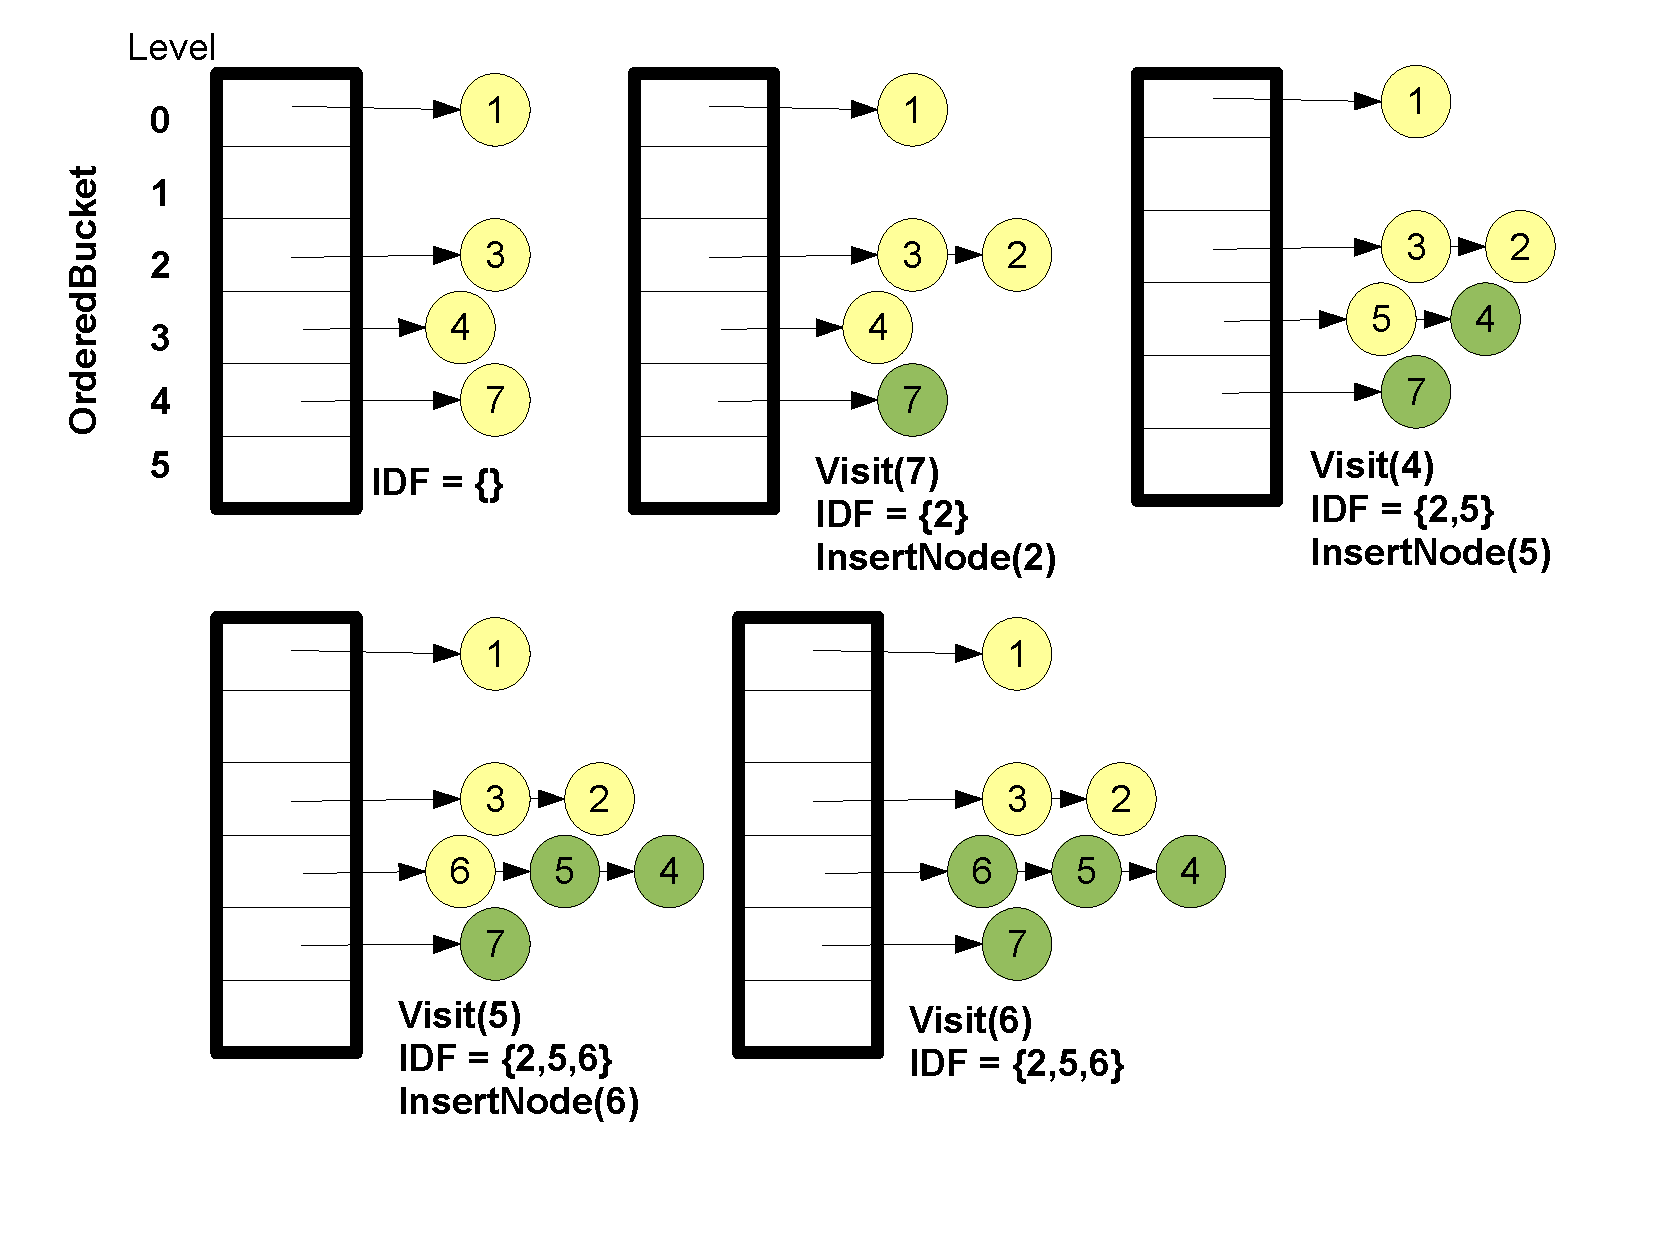
\includegraphics[scale=0.3]{sreedhargao.pdf}}
    \caption{Phases of Sreedhar and Gao's algorithm for $N_\alpha=\{1,3,4,7\}$.}
    \label{fig:sreedhargao}
    \end{figure} 

In Figure ~\ref{fig:sreedhargao}, some of the phases of the algorithm are depicted for clarity. The $OrderedBucket$
is populated with the nodes $1,3,4$ and $7$ corresponding to $N_\alpha=\{1,3,4,7\}$. The nodes are
placed in the buckets corresponding to the levels at which they appear. Hence, node 1 which appears at 
level 0 is in the zero-th bucket, node 3 is in the second bucket and so on. Since the
nodes are processed bottom-up, the first node that is visited is node 7. The successor of node 7 is node
2 and since there exists a J edge $7 \edge{J} 2$, and the $IDF$ set is empty, the $IDF$ set is updated
to hold node 2 according to step ~\ref{C:idf} of the Visit procedure. In addition, InsertNode(2) is invoked and 
node 2 is placed in the second bucket. The next node visited is node 4. The successor of node 4 which is node
5 has an incoming J edge $4 \edge{J} 5$ which results in the new $IDF = \{2,5\}$. The final $IDF$ set converges
to $\{2,5,6\}$ when node 5 is visited. Subsequent visits of other nodes do not add anything to the
$IDF$ set. An interesting case arises when node 3 is visited. Node 3 finally causes nodes 9 and 10 also 
to be visited. However, when node 10 is visited, its successor node which is node 8 and which also 
corresponds to the J edge $10 \edge{J} 8$, does not result in an update of the $IDF$ set as the level of
node 8 is higher than that of node 3.

Cytron's approach for $\phi$-placement involves a fully eager approach of constructing the entire DF graph. On the other hand Sreedhar and Gao's approach is a fully lazy approach as it constructs DF on-the-fly only when a query is encountered.
Pingali and Bilardi \cite{bilardi} suggested a middle-ground by combining both the approaches. They proposed a new representation called ADT(Augmented Dominator Tree). 
The ADT representation can be
thought as a DJ graph, where the DF sets are pre-computed for certain nodes called ``boundary nodes'' using an eager approach. For the rest of the nodes, termed ``interior nodes'', the DF needs to be computed on-the-fly as in the Sreedhar-Gao algorithm. The nodes which act as ``boundary nodes'' are detected in a separate pass. A factor $\beta$ is used to determine the partitioning of the nodes of a CFG into boundary or interior nodes by dividing the CFG into zones. $\beta$ is a number that represents space/query-time tradeoff. $\beta << 1$ denotes a fully eager approach where storage requirement for DF is maximum but query-time is faster while $\beta >> 1$ denotes a fully lazy approach where storage requirement is zero but query is slower. 

Given the ADT of a control flow graph, it is straight forward to 
modify  Sreedhar and Gao's algorithm for computing $\phi$-functions in linear time. The only modification that is needed is to ensure that we need not visit all the nodes of a sub-tree rooted at a node $y$ when $y$ is a boundary node whose DF set is already known. This change is reflected at step \ref{C:cached} of Figure~\ref{F:IDFMain}, where a subtree rooted at $y$ is visited or not visited based on whether it is a boundary node or not.


\section{Placing $\phi$-functions using Merge Sets}

In the previous section we described $\phi$-function placement algorithm in terms 
of iterated dominance frontier. There is another way to approach the problem
of $\phi$-function placement using the concept of merge relation and merge set. In this section
we will first introduce the notion of merge set and merge relation and then show
how merge relation is related to DF relation. We will then show how to compute
M (merge) graph using DJ graph and then use M graph for placing $\phi$-functions.

\subsection{Merge Set and Merge Relation}

Let us define first the notion of a {\em join} set $J(S)$
 for a given set of nodes  $S$ in a control flow
graph.\footnote{In English `join' and `merge' are synonyms, 
but unfortunately
in the literature, due to lack of  better terms, these two synonyms are used to mean
distinct but related concepts.} Consider two nodes $u$ and $v$ and distinct 
paths from $u \edge{+} w$ and $v \edge{+} w$, where $w$ is some node in the CFG. If the 
two paths meet only at $w$ then $w$ is in the join set of the nodes $\{u, v\}$. 
For instance, consider nodes 1 and 9 in Figure ~\ref{fig:cfg}(a).
The paths $1 \edge{} 2 \edge{} 3 \edge{} 8$ and $9 \edge{} 10 \edge{} 8$ meet at $8$ 
for the first time and so $\{8\} \in J(\{1,9\})$. 

Now let us define {\em merge} relation as a relation $v=M(u)$
that holds between two nodes $u$ and $v$ whenever
$v \in J(\{root, u\})$. We insert a $\phi$-function at $v$ for a variable that is assigned
only at $root$ and $u$. One can show that $J(S) = \cup_{u \in S} M(u)$ where $S \subseteq V$. Also, for any node $u \in V$, $v \in M(u)$ if and only if
there is a path $u \edge{+} v$ that does not contain $idom(v)$.  This relationship between
dominance and merge can be conveniently encoded using DJ graph and used for placing 
$\phi$-functions. First we will construct DF (Dominance Frontier) graph using DJ graph.
For each J edge $u \edge{} v$ in the DJ graph insert a new  $w \edge{J} v$ where
$w = idom (u)$ and $w$ does not strictly dominate $v$. Another way to
look at this is to insert a new J edge $w \edge{} v$ if $w = idom(u)$ and
$w.level \geq v.level$.\footnote{Recall that $w.level$ is the depth of $w$ from
$root$ of the dominator tree.} We repeatedly insert new J edges in a bottom-up fashion
over the DJ graph until no more J edges can be inserted. The resulting
DJ graph is a ``fully cached'' DJ graph. We will call the fully cached
DJ graph as the DF graph as the $DF(x) = \{t| x \edge{J} t$\}.

Next we can compute the M relation from the DF graph. 
Recall that  we insert an edge from a node $u$ to
a node $v $ if $v \in M(u)$. Using DF graph we compute
the M graph as transitive closure
using only the DF edges of the DJ graph. Now given the M graph of
a CFG we can place $\phi$-functions to a set $S \subseteq \ V$ at the neighbouring nodes of the nodes in $S$. In Figure ~\ref{fig:mgraph}, $M(4) = \{2,5,6\}$ as the nodes 2,5 and 6 are the only nodes reachable from node 4 following the DF edges. Similarly, for node 8, $M(8) = \{2,5,6,8\}$ due to these nodes being reachable from node 8 via the DF edges.

    \begin{figure}[htb]
    \centerline{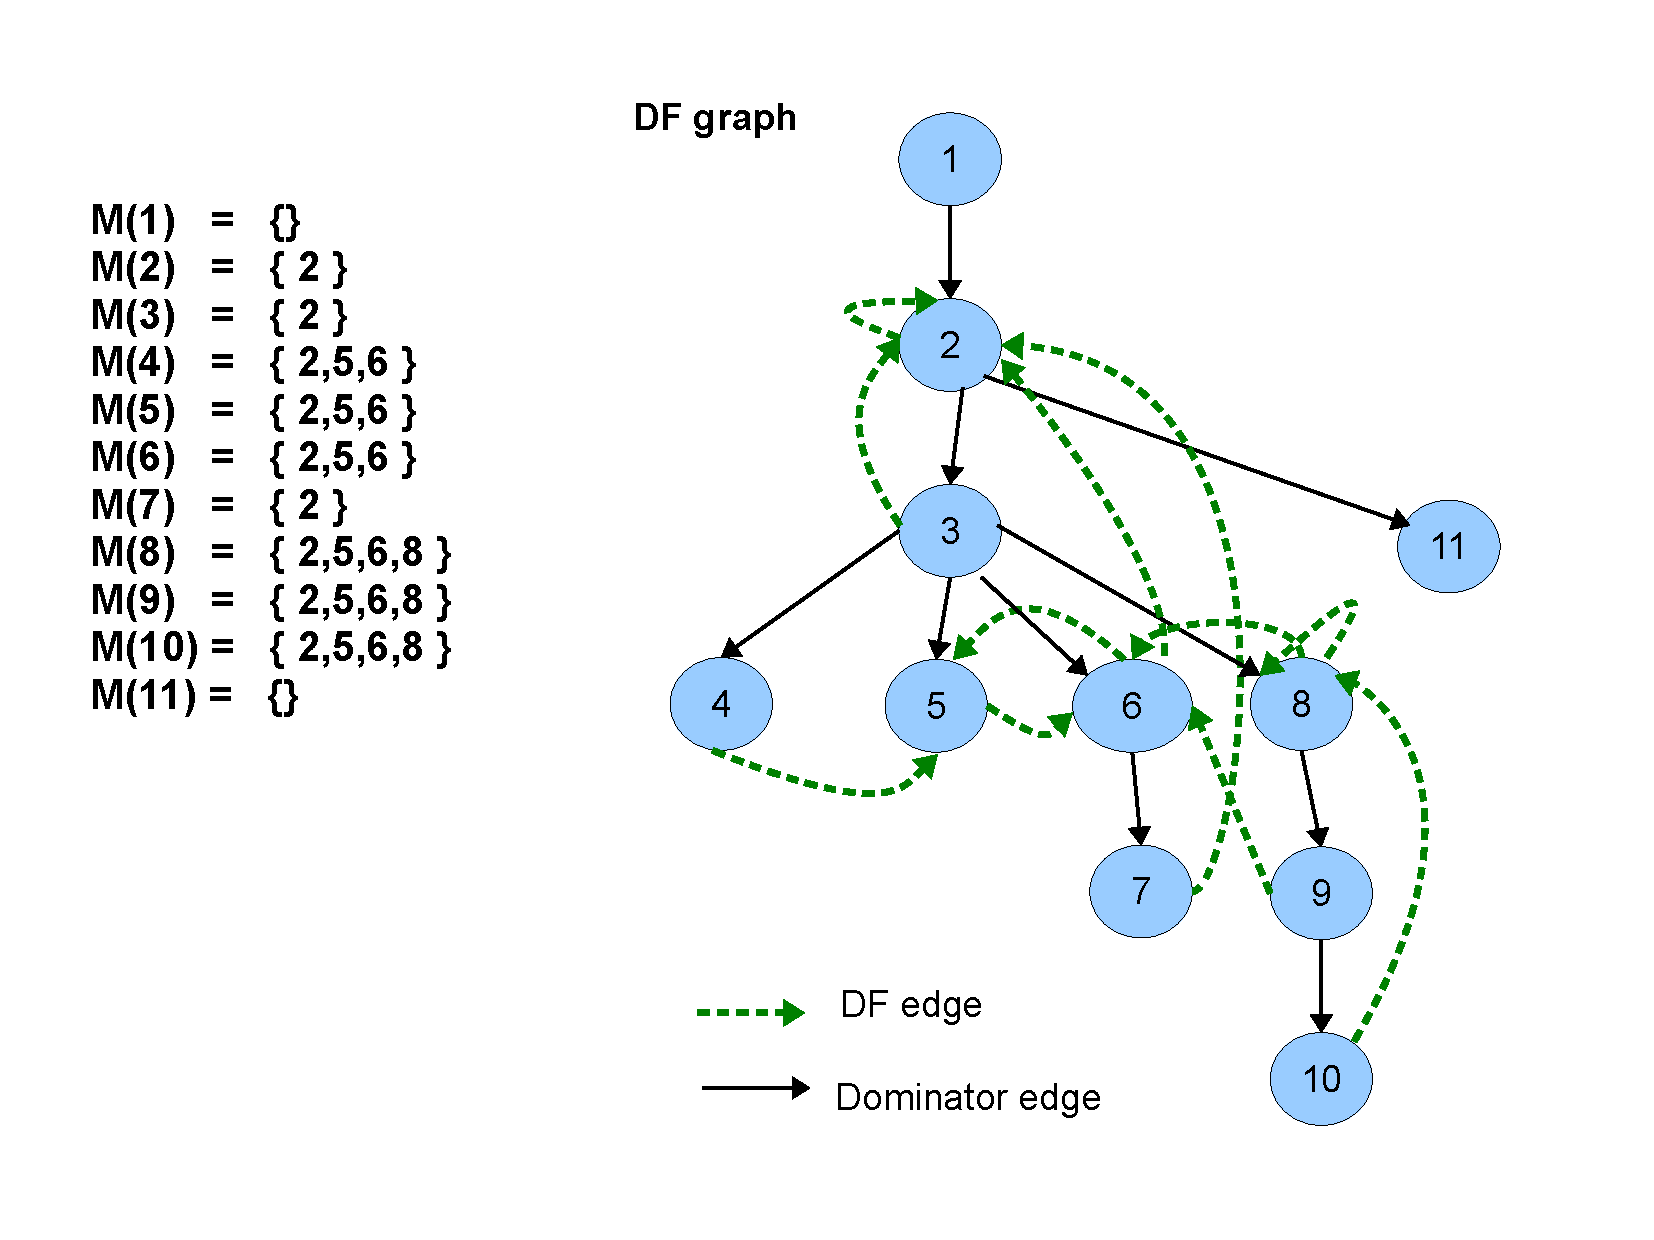
\includegraphics[scale=0.4]{mgraph_1.pdf}}
    \caption{DF graph and M sets}
    \label{fig:mgraph}
    \end{figure} 

The algorithms \cite{} for placing $\phi$-functions based on the construction of DF graph or M relation 
in the worst case can be quadratic. The merge relation is due to Pingali and Bilardi \cite{}. The DF graph and the M sets for the running example are given in Figure ~\ref{fig:mgraph}.

\subsection{Iterative Merge Set Computation}
In this section we describe a method to iteratively compute the $merge$ relation using a dataflow formulation. In the previous section we saw that the $merge$ relation can be computed using a transitive closure of the DF graph, which in turn can be computed from the DJ graph. In the algorithm proposed by Das and Ramakrishna \cite[], explicit DF graph construction or the transitive closure formation are not necessary. Instead, the same result can be achieved by formulating the $merge$ relation as a dataflow problem and solving it iteratively. For several applications, this approach has been found to be a fast and effective method to construct $M(x)$ for each node $x$ and the corresponding $\phi$-function placement using the $Mx)$ sets. 

Consider a J edge $u \edge{J} v$. Also consider all nodes $w$ s.t. $w$ dominates $u$ and $w.level \geq v.level$. For every $w$ we can set up the dataflow equation as $M(w) = M(w) \cup M(v) \cup \{v\}$. The set of dataflow equations for each node $n$ in the DJ graph can be solved iteratively using a top-down pass over the DJ graph. To check whether multiple-passes are required over the DJ graph before a fixed-point is reached for the dataflow equations, we devise an ``inconsistency condition'' stated as follows.

\paragraph{Inconsistency Condition:}

For a J edge, $u \edge{J} v$, if $u$ does not satisfy
$M(u)\supseteq M(v)$, then the node $u$ is said to be inconsistent. 

The algorithm described in the next section is directly based on the method of building
up the $M(x)$ sets of the nodes as each J edge is encountered in an iterative fashion by
traversing the DJ graph top-down. If no node is found to be {\bf inconsistent} after a single 
top-down pass, all the nodes are supposed to have reached fixed-point solutions. If some node
is found to be inconsistent, multiple passes are required till fixed-point solutions can be
reached.


\subsubsection{TopDownMergeSetComputation}

%==
\begin{figure}[!ht]
\centering
\begin{minipage}[t]{5in}
\noindent{\bf Input:} A DJ graph representation of a program.
\noindent{\bf Output:} The merge sets for the nodes.

\setcounter{linectr}{0}
Procedure TDMSCMain
\{
\begin{code}
\x1 $\forall node x \in$ DJ graph set $M(x) = \{\}$
\x1 {\it done = false};
\x1 {\bf while} ( ! {\it done} ) {\bf do}
\x2     {\it done} = TDMSC-I(DJ graph);
\x1 {\bf end while}
\end{code}
\}

Procedure TDMSC-I(DJ graph)
\{
\begin{code}
%\textbf{Algorithm: Top Down Merge Set Computation (TDMSC-I)}
%Input: $DJ$-graph
%Outputs: Complete Merge Sets for every node of the DJ graph

\x1 $RequireAnotherPass=false$;

\x1 {\bf while} (in B(readth) F(irst) S(earch) order of DJ graph) {\bf do} \label{C:bfs}
\x2      $n$ $=$ Next Node in BFS list
\x2      {\bf for} (all incoming edges to $n$) {\bf do} \label{C:jedge}

\x3          Let $e = s \edge{J} n$ , be an incoming J edge
\x3          {\bf if} ($e$ not marked visited) {\bf then}
\x4              Mark $e$ as visited 
\x4              $tmp$ $=$ $s$;
\x4              $lnode$ $=$ $NULL$;
\x4              {\bf while} $(level(tmp)\ge level(n))$ {\bf do} \label{C:mwhiles}

\x5                   $M(tmp)=M(tmp)\cup M(n)\cup \{n\}$;
\x5                   $lnode=tmp$;
\x5                   $tmp=parent(tmp)$; //dominator tree parent
\x4              {\bf end while} \label{C:mwhilee}
\x4              {\bf for} (all incoming edges to $lnode$) {\bf do} \label{C:lnode}
\x5                  Let $e'$ $=$ $s^{'} \edge{J} lnode$, be an incoming J edge
\x5                  {\bf if} ($e'$ visited) {\bf then}
\x6                     {\bf if} $(M(s') \not\supseteq M(lnode))$ {\bf then} //Check inconsistency
\x7                         $RequireAnotherPass = true$;
\x6                     {\bf end if}
\x5                  {\bf end if}
\x4              {\bf end for}
\x3          {\bf end if}
\x2     {\bf end for}
\x1 {\bf end while}
\x1 {\bf return} $RequireAnotherPass$;
\end{code}
\}
\end{minipage}
\caption{Top Down Merge Set Computation algorithm for computing Merge sets.}
\label{F:tdmsc}
\end{figure} 

The first and direct variant of the approach laid out above is termed TDMSC-I. This variant works by scanning the DJ graph in a top-down fashion as shown in step ~\ref{C:bfs}
of Figure~\ref{F:tdmsc}. All $M(x)$ sets are set to the null set before the initial pass of TDMSC-I. The $M(x)$ sets computed in a previous pass are carried over if a subsequent pass is required. 

The DJ graph is visited
level-by-level. During this process, for each node $n$ encountered, if there is an {\bf incoming}
J edge $s \edge{J} n$ to $n$ as in step ~\ref{C:jedge}, then a separate bottom-up pass starts at 
step ~\ref{C:mwhiles}. This bottom-up pass traverses all nodes $w$ s.t. $w$ dominates $s$ and $w.level \geq s.level$,
updating the $M(w)$ values using the aforementioned dataflow equation. Step ~\ref{C:lnode} is used for
inconsistency check. $RequireAnotherPass$ is set to true only if a fixed point is not reached
and the inconsistency check succeeds for some node.

There are some subtleties in the algorithm that should be noted. Step ~\ref{C:lnode} of the algorithm visits incoming edges to $lnode$ only as $lnode$ is at the same level as $n$, which is the current level of inspection and the incoming edges to $lnode$'s posterity are at a level greater than that of node $n$ and are unvisited yet. 

Here, we will briefly walk through TDMSC-I using the DJ graph of Figure ~\ref{fig:cfg}(b). Moving top-down over the graph, the first J edge encountered is $7 \edge{J} 2$. As a result, a bottom-up climbing of the nodes happen, starting at node $7$ and
ending at node $2$ and the merge sets of these nodes are updated so that $M(7) = M(6) = M(3) = M(2) = \{2\}$. The next J edge
to be visited can be any of $4 \edge{J} 5$, $5 \edge{J} 6$ or $6 \edge{J} 5$ at $level = 3$. Assume it is $5 \edge{J} 6$. This results in $M(5) = M(5) \cup M(6) \cup \{6\} = \{2,6\}$. Now, let $6 \edge{J} 5$ be visited. Hence, $M(6) = M(6) \cup M(5) \cup \{5\} = \{2,5,6\}$. At this point, the {\bf inconsistency check} comes into picture for the edge $6 \edge{J} 5$ as $5 \edge{J} 6$ is another J edge that is already visited and is an incoming edge of node $6$. Checking for $M(5) \supseteq M(6)$ fails, implying that the $M(5)$ needs to be computed again. This is done in a separate pass as suggested by the {\it RequireAnotherPass} value of true. In a second iterative pass, the J edges are visited in the same order. Now, when $5 \edge{J} 6$ is visited, 
$M(5) = M(5) \cup M(6) \cup \{6\} = \{2,5,6\}$ as 
the current $M(5) = \{2,6\}$ 
and $M(6) = \{2,5,6\}$. On a subsequent visit of $6 \edge{J} 5$, $M(6)$ is also set to $\{2,5,6\}$. The inconsistency does not appear any more and the algorithm proceeds to handle the edges $4 \edge{J} 5$, $9 \edge{J} 6$ and $10 \edge{J} 8$ which have
also been visited in the earlier pass. TDMSC-I is invoked repeatedly by a different function
which calls it in a loop till {\it RequireAnotherPass} is returned as $false$ as shown in the procedure TDMSCMain.

\subsubsection{TDMSC-II}

TDMSC-II is an improvement to algorithm TDMSC-I. This improvement is fueled by the observation that for an inconsistent node $u$, the merge sets of all nodes $w$ s.t. $w$ dominates $u$ and $w.level \geq u.level$,
can be locally corrected for some special cases. This
heuristic works very well for certain class of problems -- especially for CFGs with DF graphs having cycles consisting of a few edges. This eliminates extra passes as an inconsistent node is made consistent immediately on being detected. For details of this algorithm refer to \cite{}.

\subsubsection { Final $\phi$-function placement using Merge Sets }
Once the $Merge$ relation is computed for the entire CFG, placing $\phi$ is a straightforward application of the $M(x)$ values for a given $N_{\alpha}$, as shown in Figure ~\ref{F:phip}.
\begin{figure}[!ht]
\centering
\begin{minipage}[t]{5in}
\noindent{\bf Input:} A CFG with Merge sets computed and $N_{\alpha}$.
\noindent{\bf Output:} Blocks augmented by $\phi$-functions for the given $N_{\alpha}$.

\setcounter{linectr}{0}

Procedure $\phi$-placement for $N_{\alpha}$
\{
\begin{code}
\x1 {\bf for} ($\forall n \in N_{\alpha}$) {\bf do}
\x2   {\bf for} ($\forall n^{'} \in M(n)$) {\bf do}
\x3       Add a $\phi$ for $n$ in $n^{'}$ if not placed already
\x2   {\bf end for}
\x1 {\bf end for}
\end{code}
\}
\end{minipage}
\caption{$\phi$-placement using $Merge$ sets}
\label{F:phip}
\end{figure} 

\section{Computing Iterated Dominance Frontier Using Loop Nesting Forests}
    This section illustrates the use of {\bf loop nesting forests} for construction of the iterated
    dominance frontier (IDF) of a set of vertices in a CFG, which may contain both reducible as well as
    irreducible loops.

    \subsection{Loop nesting forest}
     Loop nesting forest is a data structure that respresents the loops in a CFG
    and the containment relation between them. Loop nesting forest has been defined formally in [tobequoted]. However, while there is a fairly accepted notion of
    loop nesting forest in a reducible graph \cite{morgan_book}, there is less agreement about their
    definition in arbitrary graphs. Steensgard \cite{steensgard}, Sreedhar \cite{sreedhar} and Havlak
    \cite{havlak} all provide different definitions which have merits under different situations. 
    For the example shown in Figure ~\ref{fig:lnf}(a) the loops with backedges $11 \rightarrow 9$ and
    $12 \rightarrow 2$ are both reducible loops. The corresponding loop nesting forest shown in Figure ~\ref{fig:lnf}(b), consists of two loops
    with their header nodes being $2$ and $9$. 
    The loop with header node $2$ contains the loop with header node $9$.

    \begin{figure}[htb]
    \centerline{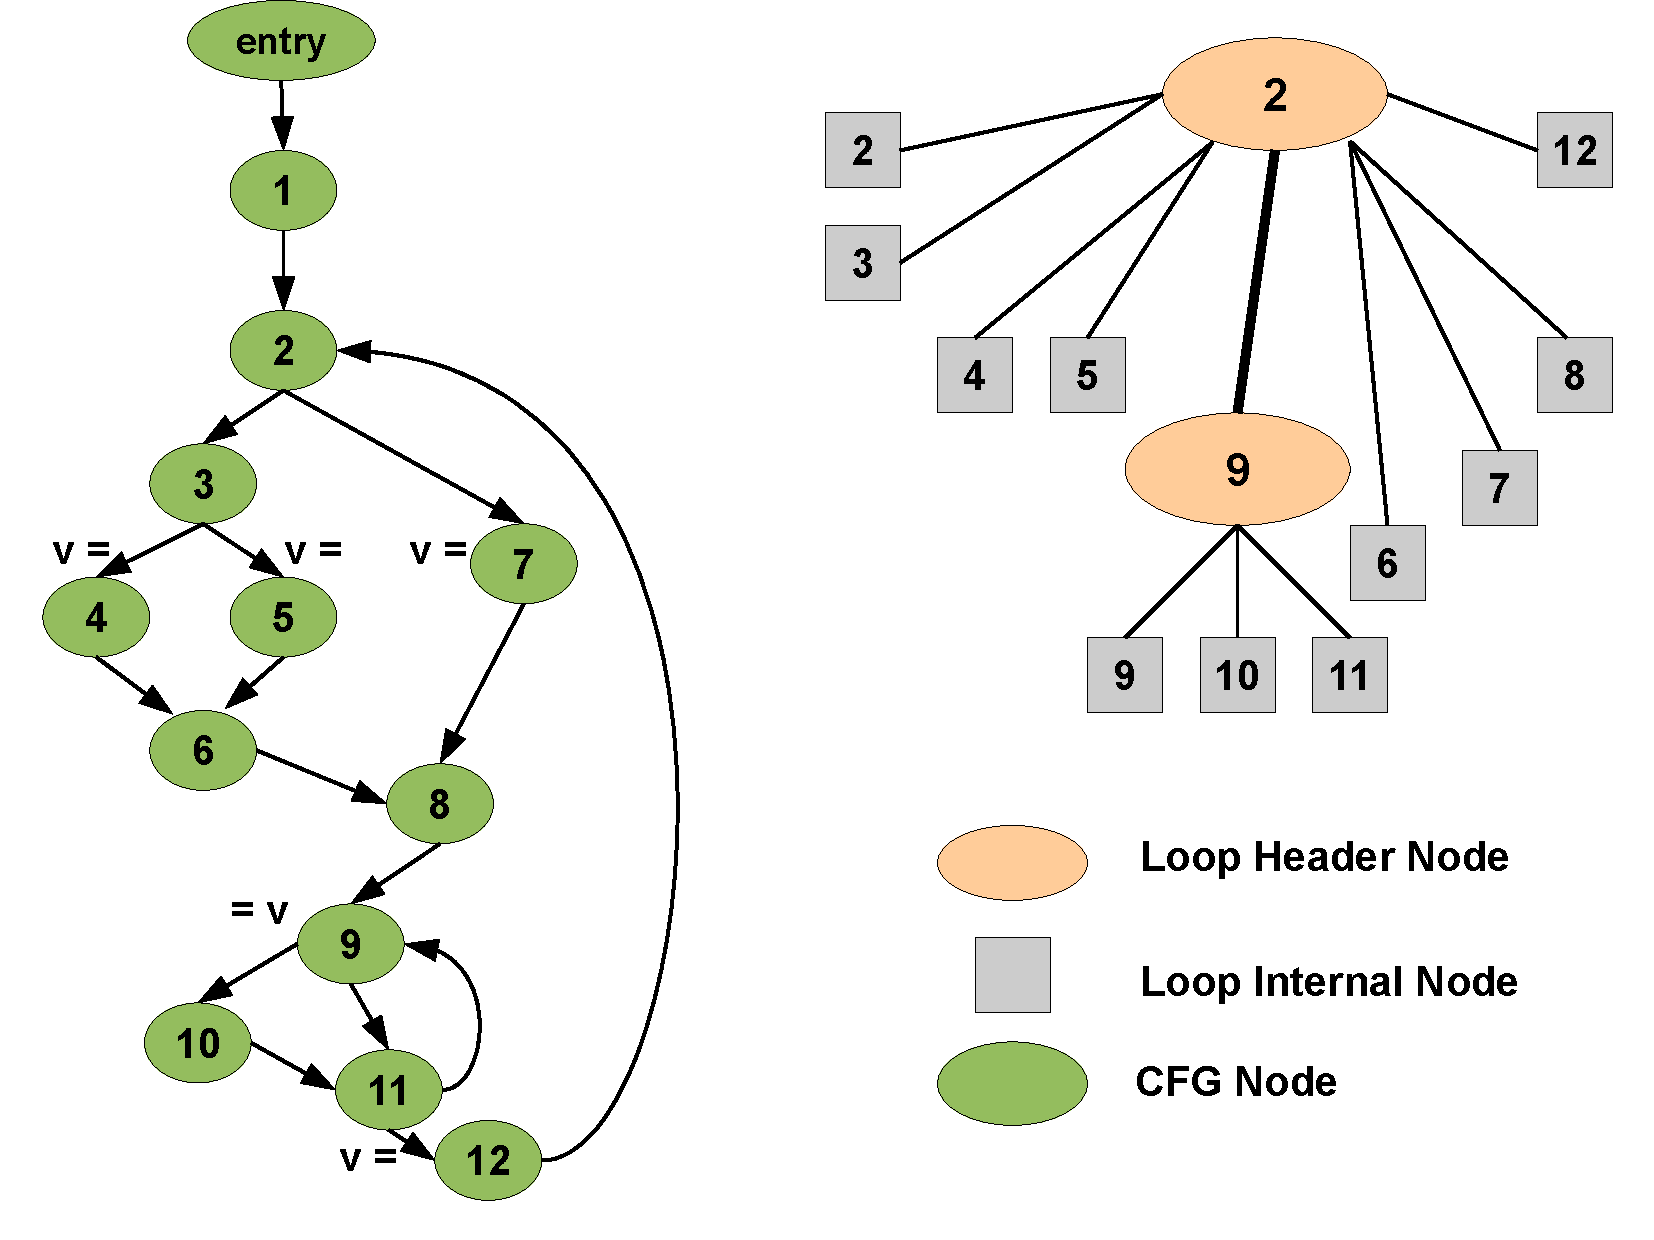
\includegraphics[scale=0.3]{lnfred.pdf}}
    \caption{An example (a) CFG and (b) IDF Computation Using Loop Nesting Forest }
    \label{fig:lnf}
    \end{figure} 


    \subsection{Main Algorithm}
    
Let us say that a definition node $d$ ``reaches'' another node $u$ if there is a path in the graph from $d$ to $u$ which does not contain any definition node ( for variable $v$ ) other than $d$. If at least two definitions reach a node $u$, then $u$ belongs to $IDF(X)$ where $X$ consists of these definition nodes. This suggests the algorithm in Figure ~\ref{F:ramaIDF}. According to the algorithm, for a given $N_{\alpha}$, we can compute $IDF(N_{\alpha})$ as follows:
\begin{itemize}
\item { Initialize IDF to empty set }
\item { Using topological order compute the subset of $IDF(N_{\alpha})$ that can reach a node using forward dataflow }
{\item} {Add a node to IDF if it is reachable from multiple nodes}
\end{itemize}  

    For Figure ~\ref{fig:lnf}, the acyclic version of the graph $G$ termed $G_{ac}$ is formed by dropping
    the backedges $11 \rightarrow 9$ and $12 \rightarrow 2$. Also, $entry(G) = \{entry\}$ where $entry$ is a specially designated node that is root of the CFG.
    For the definitions of $v$ in nodes $4,5,7$ and $12$ in Figure ~\ref{fig:lnf}, 
    the subsequent nodes where multiple definitions reach turn out to be at $6$ and $8$. For node $6$
    any one of two definitions in nodes $4$ or $5$ can reach. For node $8$, it can be either the
    definition from node $7$ or one of $4$ or $6$.
    Note that the backedges do not exist in the acyclic
    graph and hence node 2 is not part of the IDF set. We will see later how the IDF set for the entire
    graph is computed by factoring in the contribution of the backedges. 



    %\begin{figure}[htb]
    %\centerline{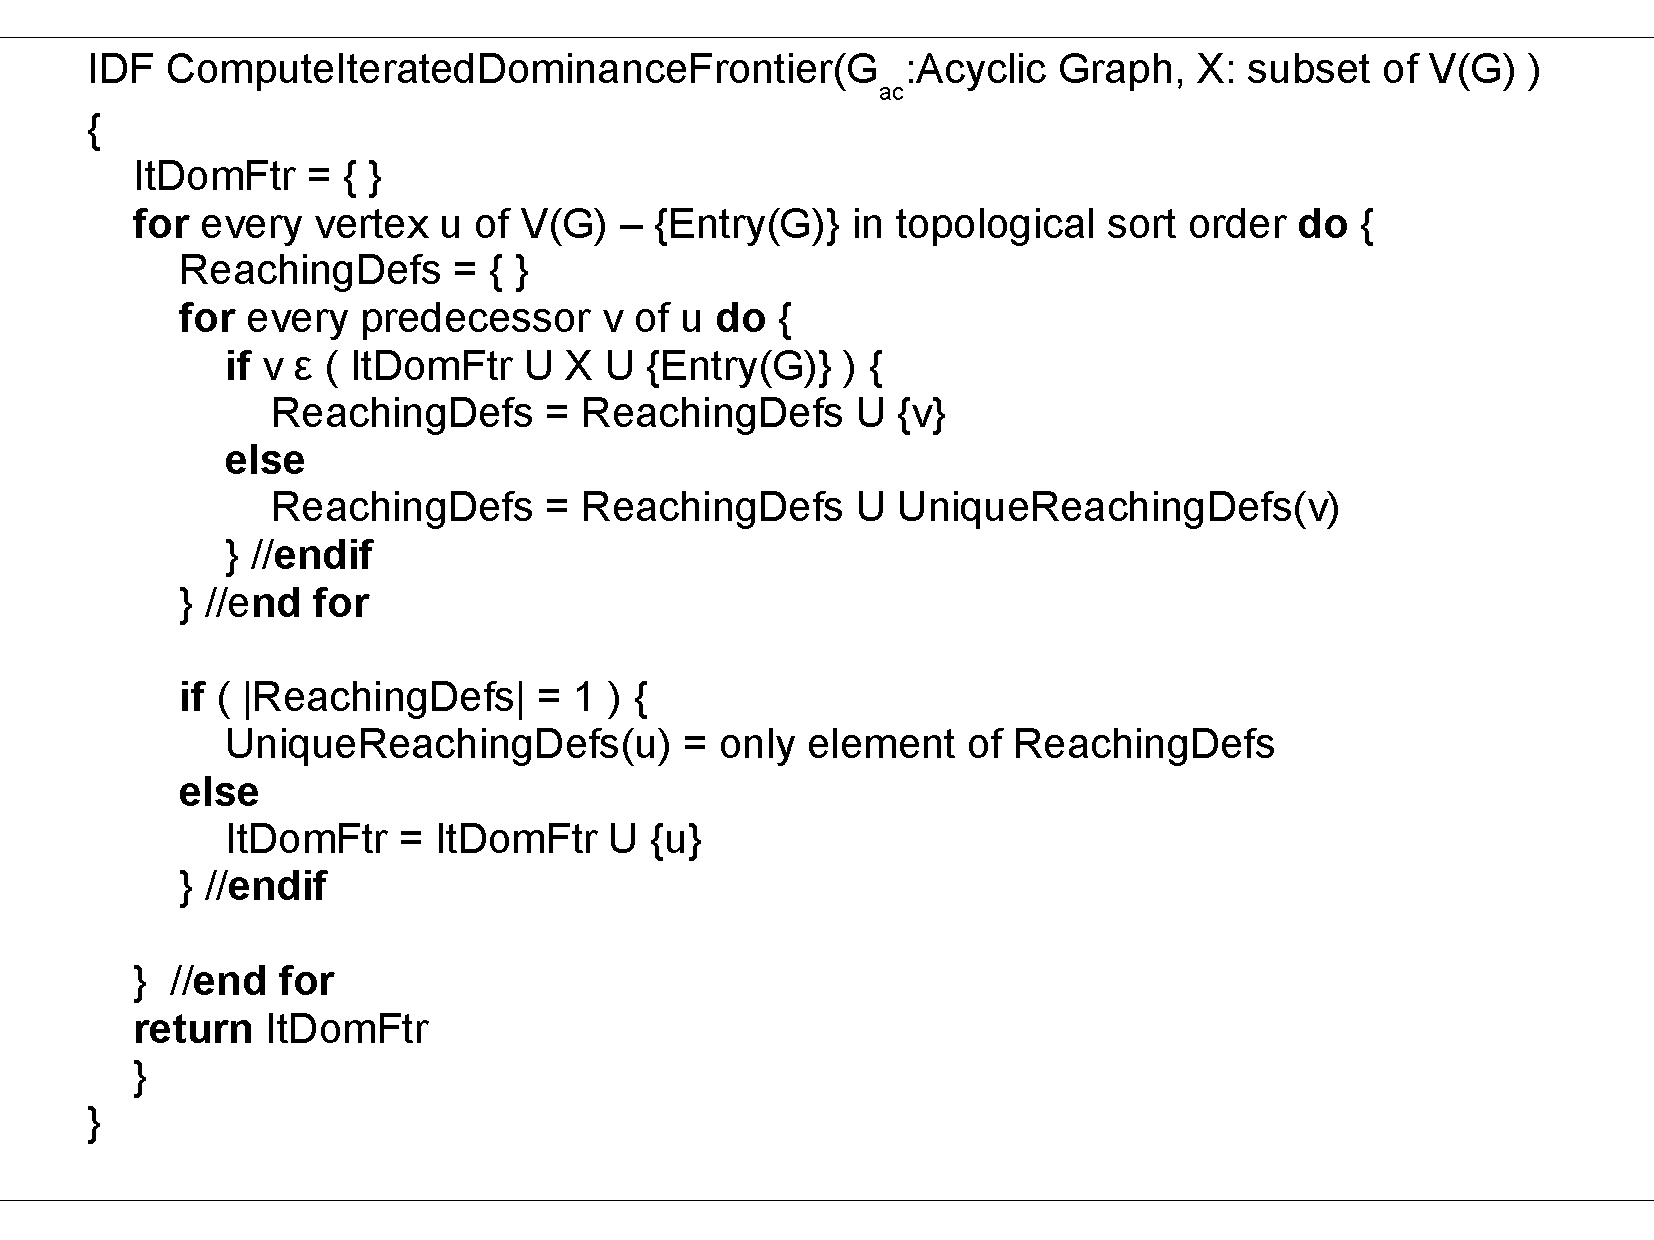
\includegraphics[scale=0.3]{idfcode.pdf}}
    %\caption{Pseudocode for computing IDF of an acyclic graph }
    %\label{fig:idfcode}
    %\end{figure}  
    
   \begin{figure}[!ht]
   \centering
  \begin{minipage}[t]{5in}
  \noindent{\bf Input:} An acyclic CFG $G_{ac}$, $X$: subset of $V(G)$.
  \noindent{\bf Output:} The set $IDF(X)$.
  \setcounter{linectr}{0}

    Procedure ComputeIteratedDominanceFrontier($G_{ac}$:Acyclic graph,$X$: subset of $V(G)$)
    \{
    \begin{code}

    \x1 $IDF = \{\}$; 
    \x1 $\forall$ $node$ of $V(G)$, $UniqueReachingDefs(node)$ = \{ \};
    \x1 {\bf for} $\forall u$ of $V(G) - entry(G)$ in topological sort order {\bf do} \{ 
    \x2    $ReachingDefs = \{ \}$; 
    \x2    {\bf for} $\forall$ predecessor $v$ of $u$ {\bf do} \{ 
    \x3      {\bf if} $v \in$ ( $IDF \cup X \cup entry(G)$ ) {\bf then} 
    \x4         $ReachingDefs = ReachingDefs \cup \{v\}$; \label{C:rdf}
    \x3      {\bf else} 
    \x4         $ReachingDefs = ReachingDefs \cup UniqueReachingDefs(v)$; \label{C:urdf}
    \x3      {\bf end if} 
    \x2   {\bf end for} 
    \x2   {\bf if} ( $\|ReachingDefs\|$ == 1 ) {\bf then} \label{C:onerd}
    \x3      $UniqueReachingDefs(u) = $ only element of $ReachingDefs$; 
    \x2   {\bf else} 
    \x3       $IDF = IDF \cup \{u\}$; \label{C:ridf}
    \x2   {\bf end if}    
    \x1 {\bf end for} 
    \x1 {\bf return} $IDF$;   
     
    \end{code}
    \}
 
  \end{minipage}
  \caption{Ramalingam's algorithm for computing the IDF of an acyclic graph.}
  \label{F:ramaIDF}
  \end{figure}

    We will walk through some of the steps of this algorithm for $IDF(\{4,5,7,12\})$. We will start at
    vertex 4. For this vertex, ${\it predecessors} = \{3\}$. But as $3 \notin IDF \cup X \cup \{entry\}$, 
    ${\it ReachingDefs} = {\it UniqueReachingDefs}(3)$ according to step ~\ref{C:urdf}. Hence, 
    ${\it ReachingDefs} = \{entry\}$. As $\|{\it ReachingDefs}\|$ equals 1, 
    ${\it UniqueReachingDefs}(4) = \{entry\}$.
    The same logic applies for vertices 5 and 7, and so, 
    ${\it UniqueReachingDefs}(5) = {\it UniqueReachingDefs}(7) = \{entry\}$.
    For vertex 6, ${\it predecessors} = \{4,5\}$.
    Since both vertices 4 and 5 belong to $X$, according to step ~\ref{C:rdf}, 
    ${\it ReachingDefs} = \{4,5\}$.
    As $\|{\it ReachingDefs}\| \neq 1$, according to step ~\ref{C:ridf}, $IDF = \{6\}$.
    Following similar arguments, $IDF = \{6,8\}$, when node 8 is visited. When the rest of the vertices
    are visited, the IDF set remains unchanged. 

    How can the algorithm to find IDF for acyclic graphs be extended to handle reducible graphs? 
    A reducible graph can be
    decomposed into an acyclic graph and a set of backedges. The contribution of backedges to the
    iterated dominance frontier can be identified by using the loop nesting forest. If a vertex $u$
    is contained in a loop then $IDF(u)$ will contain the loop header. For any vertex $u$, let $HLC(u)$
    denote the set of loop headers of the loops containing $u$. Given a set of vertices $X$, it turns
    out that $IDF(X) = HLC(X) \cup IDF_{ac}(X \cup HLC(X))$ where $IDF(X)$ and $IDF_{ac}$
    denote the IDF over the original graph $G$ and the acyclic graph $G_{ac}$ respectively. Reverting
    back to Figure ~\ref{fig:lnf} we see that in order to find the $IDF$ for the nodes where the variable 
    $v$ is defined, we need to evaluate $IDF(\{4,5,7,12\})$. Firstly, we would need to evaluate 
    $IDF_{ac}(\{4,5,7,12\} \cup HLC(\{4,5,7,12\}))$. $HLC(\{4,5,7,12\}) = \{2\}$ as all these nodes are contained 
    in a single loop with header $2$. Hence, we would need to find $IDF_{ac}(\{2,4,5,7,12\})$ which turns
    out to be the set $\{6,8\}$. Finally, $IDF(\{4,5,7,12\}) = HLC(\{4,5,7,12\}) \cup \{6,8\} = \{2,6,8\}$.
 
    %\noindent
    \begin{figure}[htb]
    \centerline{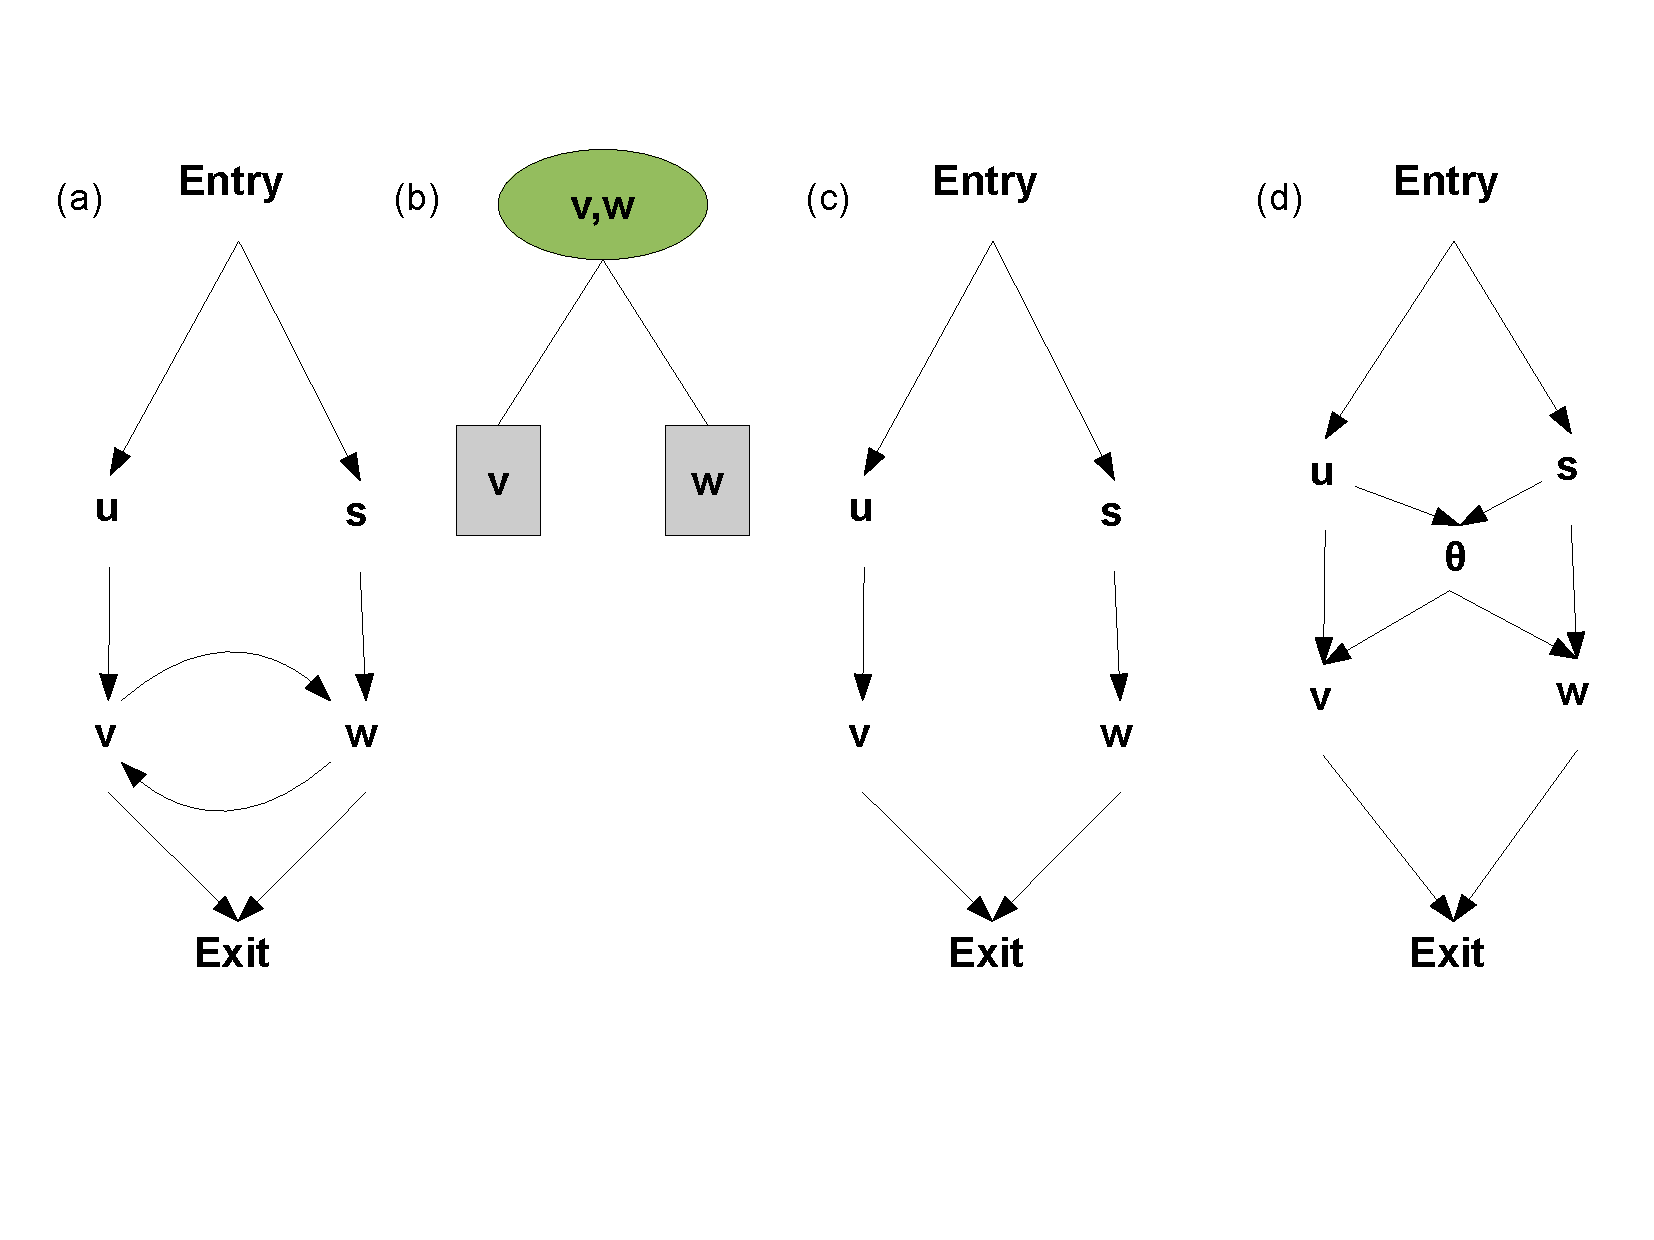
\includegraphics[scale=0.3]{irred.pdf}}
    \caption{(a) An irreducible graph (b) The Loop Nesting Forest (c) The acyclic subgraph (c) Transformed
    graph}
    \label{fig:irred}
    \end{figure} 
 
    Now that we have shown how IDF can be computed for graphs with reducible loops using 
    loop nesting forests, we will briefly touch
    upon how graphs containing irreducible loops can be handled. The insight behind the implementation
    is to transform the irreducible loop in such a way that an acyclic graph is created from the loop
    without changing the dominance properties of the nodes. Referring to Figure ~\ref{fig:irred}, we see 
    that the irreducible loop comprising of nodes $v$ and $w$ in (a) can be transformed to the acyclic
    graph in (c) by removing the edges between nodes $v$ and $w$ that create the irreducible loop. 
    We can now create a new dummy node $\theta$ and add edges from the predecessor of all
    the header nodes of the cycles of the irreducible graph to $\theta$, 
    as well as add edges from $\theta$ to all the 
    header nodes. This results in additional edges from $u$ and $s$ which are the predecessors of the
    header nodes $v$ and $w$ respectively to $\theta$. In addition, extra edges are added from $\theta$
    to the header nodes $v$ and $w$.The transformed graph is shown in (d). Following this transformation, 
    computing IDF for the nodes 
    in the original irreducible graph translates to computing IDF for the transformed graph. Since this
    graph is acyclic, the algorithm depicted in Figure ~\ref{F:ramaIDF} can be applied by noting the
    loop nesting forest structure as shown in (b). The crucial observation that allows this transformation 
    to create an equivalent acyclic
    graph is the fact that the dominator tree of the transformed graph remains identical to the
    original graph containing an irreducible cycle. One of the drawbacks of the transformation is the
    possible explosion in the number of dummy nodes and edges for graphs with many irreducible cycles as
    a unique dummy node needs to be created for each irreducible loop. However, such cases may be rare
    for practical applications.

    \section{Summary}
    This chapter provides an overview of some advanced construction algorithms
    for SSA. These include the first proposed linear-time algorithm by Sreedhar using the concept of
    DJ graphs, the merge relation by Pingali and Bilardi, a DJ graph and merge
    set based algorithm by Das and Ramakrishna and finally an algorithm by Ramalingam based on the concept
    of loop nesting forests. Though all these algorithms claim to be better than the original CFR algorithm, 
    they are difficult to compare due to the unavailability of these algorithms in a common compiler framework.
    However, some of these algorithms are known to perform better than CFR for several well-known benchmarks.


